\section{Design of CUDA Kernels}
\label{2017-gje-block-jacobi:sec:s3-kernel}

In~\cite{Anzt:2017:BGE:3026937.3026940} we designed a set of routines
for the generation and application of block-Jacobi preconditioners
via variable-size BGJE.
In this section we review the key concepts in~\cite{Anzt:2017:BGE:3026937.3026940},
and introduce several improvements to further accelerate both the 
generation and application of the preconditioner.

The generation of an inversion-based block-Jacobi preconditioner can be 
decomposed into three distinct steps:
1) extraction of the diagonal blocks; 2) inversion of {these blocks};
and 3) insertion of the inverse blocks into the preconditioner matrix.
We visualize these steps for non-uniform block sizes in Figure~\ref{2017-gje-block-jacobi:fig:batchedgje}.
The three steps can be realized as three separate CUDA kernels,
or in terms of a single kernel doing all steps in sequence.
The experimental results in~\cite{Anzt:2017:BGE:3026937.3026940}
suggest that, in general,
merging all operations into a single kernel results in higher performance.
A reason for this is the reduced memory transfer,
as realizing the operations in a single kernel avoids the main memory accesses that 
are necessary to transfer data {between separate kernels}.
In this paper we therefore focus on merged kernels for generating block-inverse matrices.

The question of how to identify a convenient block structure for a given 
coefficient matrix and an upper bound limiting the size of the diagonal blocks remains 
outside the focus of this paper.
Here, for all experiments we use the supervariable blocking routine
available in MAGMA-sparse~\cite{magma}.

\begin{figure}[t]
\begin{center}
\begin{tabular}{c}
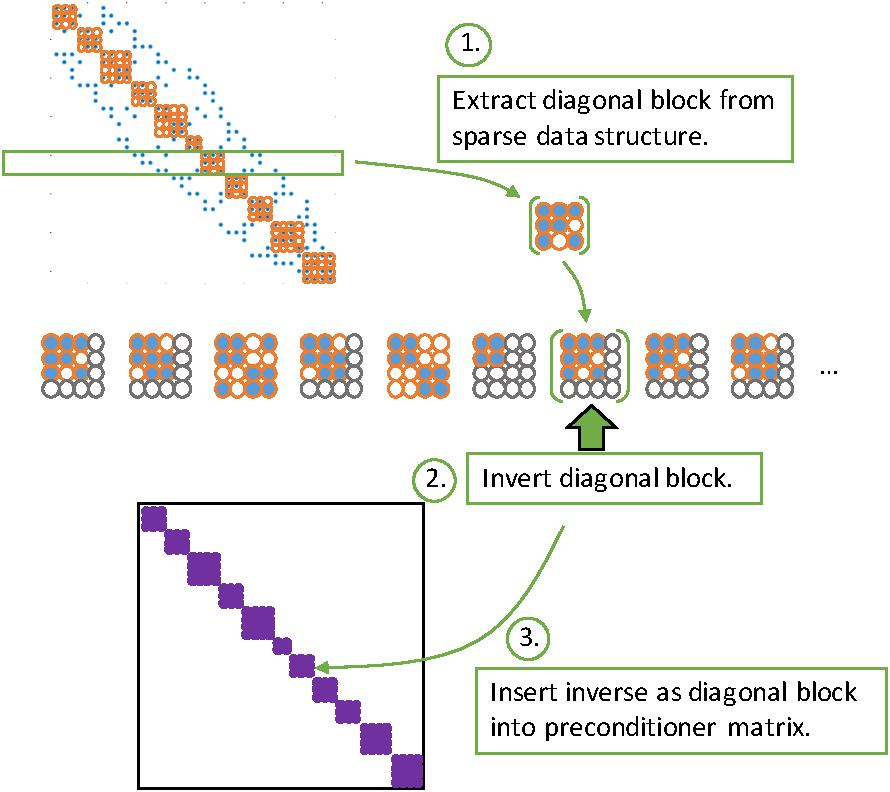
\includegraphics[width=.65\columnwidth]{plots/scheme_inversion}
\end{tabular}
\end{center}
\caption
[Generation of the block-Jacobi preconditioner]
{Generation of the block-Jacobi preconditioner: 1) data extraction; 2) variable-size BGJE; 3) data insertion.
The block structure is indicated with orange circles, the original nonzero pattern with blue dots, 
    {and} the block inverses with purple circles.
}
\label{2017-gje-block-jacobi:fig:batchedgje}
\end{figure}

\subsection{Variable-size batched Gauss-Jordan elimination}
\label{2017-gje-block-jacobi:subsec:s3-inversion}

The central operation in the generation of an 
inversion-based block-Jacobi preconditioner
is the inversion of the diagonal blocks in $D$.
These blocks are all square, of small dimension, and independent.
In~\cite{Anzt:2017:BGE:3026937.3026940}
we designed a variable-size BGJE routine
that assigns one CUDA warp (a group of 32 threads) 
to invert each diagonal block.
The kernel is launched on a grid with the number of warps 
covering the number of diagonal blocks.
Within a warp, parallelism is realized by each thread handling one row
of the diagonal block.
This limits the scope of the kernel to matrix batches where no matrix
is of dimension larger than 32.
As blocks of larger dimension are rarely {encountered} in the context
of block-Jacobi preconditioning, the variable-size batched GJE
kernel perfectly fits this application scope~\cite{Anzt:2017:BGE:3026937.3026940}.

Handling the inversion with a single warp allows us to
use two recent features of NVIDIA's GPU architectures:
increased register count and warp shuffle instructions.
In some detail, the data required by each thread
(up to 32 data elements belonging to the matrix row)
is first read into registers;
the inversion is then computed using this data and communication occurs via the warp shuffle instruction
(avoiding main memory access during the inversion process);
and finally, the computed inverse is written back to main memory.
In general, even though the diagonal blocks are sparse,
their inverses are dense.
We therefore handle and store the diagonal blocks in dense format during the complete inversion process.

The pivoting process ensuring numerical stability requires to identify the pivot element, 
see line~8 in Figure~\ref{2017-gje-block-jacobi:fig:gje2}. 
Since the matrix is distributed row-wise among the threads,
this requires a parallel reduction.
We realize this step via warp shuffles.
The same type of shuffles is also used to distribute the contents
of the current pivot row \texttt{Di(ipiv, k)}
required for the operations in lines~12--15.

\vspace*{1ex}
\noindent
\textbf{Multiple problems per warp.}
The variable-size BGJE presented in~\cite{Anzt:2017:BGE:3026937.3026940}
assigns one warp to each diagonal block. 
{In that work, diagonal} blocks of size $k<32$ were padded with dummy values to that dimension and the
threads only execute the first $k$ iterations of the GJE algorithm.
Obviously, for small blocks, 
this wastes a significant part of the computational resources,
as most of the threads then operate on dummy data.
{In this work, we} improve the algorithm by 
allowing one warp to handle multiple small problems simultaneously.
Concretely, {let $k_m$ denote the size of the largest block in the matrix batch
and $p_m$ stand for the smallest power of 2 such that $p_m \geq k_m$;
then, in our new approach, each warp processes $32 / p_m$ blocks.
Proceeding in this manner,} each group of $p_m$ threads -- we call it {\it sub-warp} -- 
is assigned to one problem.
The first $k_m$ threads in the sub-warp compute the inverse of a block
of size $k \leq k_m$ by padding it with dummy values to size $k_m$,
and computing {only} the first $k$ steps of the inversion procedure.
The rest of the threads in the sub-warp remain idle.
The reason for choosing $p_m$
as the sub-warp size is
that the CUDA ecosystem supports warp shuffles for these sizes.
Using $k_m$ instead of $p_m$ would require additional operations 
to calculate the thread index.
Finally, we do not consider ``packing'' blocks of different sizes into one warp
(e.g.,
one warp could process blocks of sizes 15 and 17),
as this {would require} a preprocessing step in order to determine
which warp can process which set of blocks. {Furthermore, 
it would} also result in thread divergence between the two parts of the warp.

\subsection{Data extraction from the sparse coefficient matrix}
\label{2017-gje-block-jacobi:subsec:s3-extraction}

As BGJE expects a collection of small dense blocks as input,
these blocks need to be extracted from the sparse coefficient matrix
stored in CSR format~\cite{saad}.
We next review the two extraction strategies we implemented and compared 
in~\cite{Anzt:2017:BGE:3026937.3026940}.


The first approach, named {\it cached extraction}, is a straight-forward method
where each thread traverses a single matrix row,
(specifically, the row whose values will be required by this thread during inversion process,)
and extracts the elements that lie on the corresponding diagonal block.
Since the CSR format is designed to favor accessing sparse matrix by rows, 
({i.e., it keeps the matrix entries in row-major order,})
this will most likely result in non-coalescent memory 
access.
Furthermore, an unbalanced nonzero distribution in the coefficient matrix
inevitably incurs load imbalance, as threads operating on short rows will remain idle while the 
remaining threads extract the data from their rows.
Both effects impair the performance of the extraction step.


As a response to these issues, in~\cite{Anzt:2017:BGE:3026937.3026940} we proposed 
an alternative 
{\it shared extraction} method.
The key idea is to eliminate non-coalescent memory access and
(potential) load imbalance at the cost of using shared memory.
Precisely, all threads of the warp collaborate on the extraction of the block
by accessing each row containing part of the block in a coalesced mode
(see Figure~\ref{2017-gje-block-jacobi:fig:memtransact}).
The diagonal block is then converted to dense format and stored 
into shared memory by writing the extracted 
values into the appropriate locations in shared memory, see right-hand side  in Figure~\ref{2017-gje-block-jacobi:fig:memtransact}.
Once the extraction of a block is completed,
each thread reads the values of the row assigned to it from shared memory.
This strategy makes all memory accesses coalescent
and alleviates load imbalance.
The shared memory usage, however, can constrain
the number of warps active per multiprocessor.
On ``older'' GPU architectures we observed that the shared extraction
strategy can result in lower performance due to this issue.

\vspace*{1ex}
\noindent
\textbf{Reduced usage of shared memory.}
We improve the situation by radically reducing the amount of shared memory employed in the
shared extraction step.
This is possible because the inverse of a matrix $A$ can be computed
by first obtaining the inverse of $A^T$ and then transposing the result
(i.e., $((A^T)^{-1})^T = A^{-1}$).
Extracting the transpose of the diagonal block is much easier
as the $i$-th elements of all columns are 
available as soon as the $i$-th row is extracted to shared memory.
This means that all threads can already read the $i$-th row-value
of the transposed block into registers before proceeding with the extraction
of the next row.
Thus, the extraction of the transpose block
from the sparse matrix structure can be ``interleaved'' with
{the retrieval of} the values from shared memory into the registers.
As a result, the same shared memory locations
used to store row $k$ of the diagonal block
can be re-used in the following step of the extraction.
This reduces the total {amount of} shared memory required to 
{that necessary to keep} a single row of the diagonal block.

In case multiple blocks are assigned to each warp,
a straight-forward extension of the strategy is to
{let each sub-warp extract} the block assigned to it.
This would, however, result in non-coalesced memory access.
Coalesced memory access can be preserved
by extracting all blocks handled by the warp in sequence,
using all threads of the warp and {enough shared memory to store one}
row of the largest matrix in the batch.

After the inversion of a diagonal block is completed,
the result is written back to main memory.
Realizing the afore-described extraction step in reverse order,
we store the inverse of the transposed block in transposed mode
 -- which is the inverse of the original block.

\begin{figure}[t]
\begin{center}
\begin{tabular}{r}
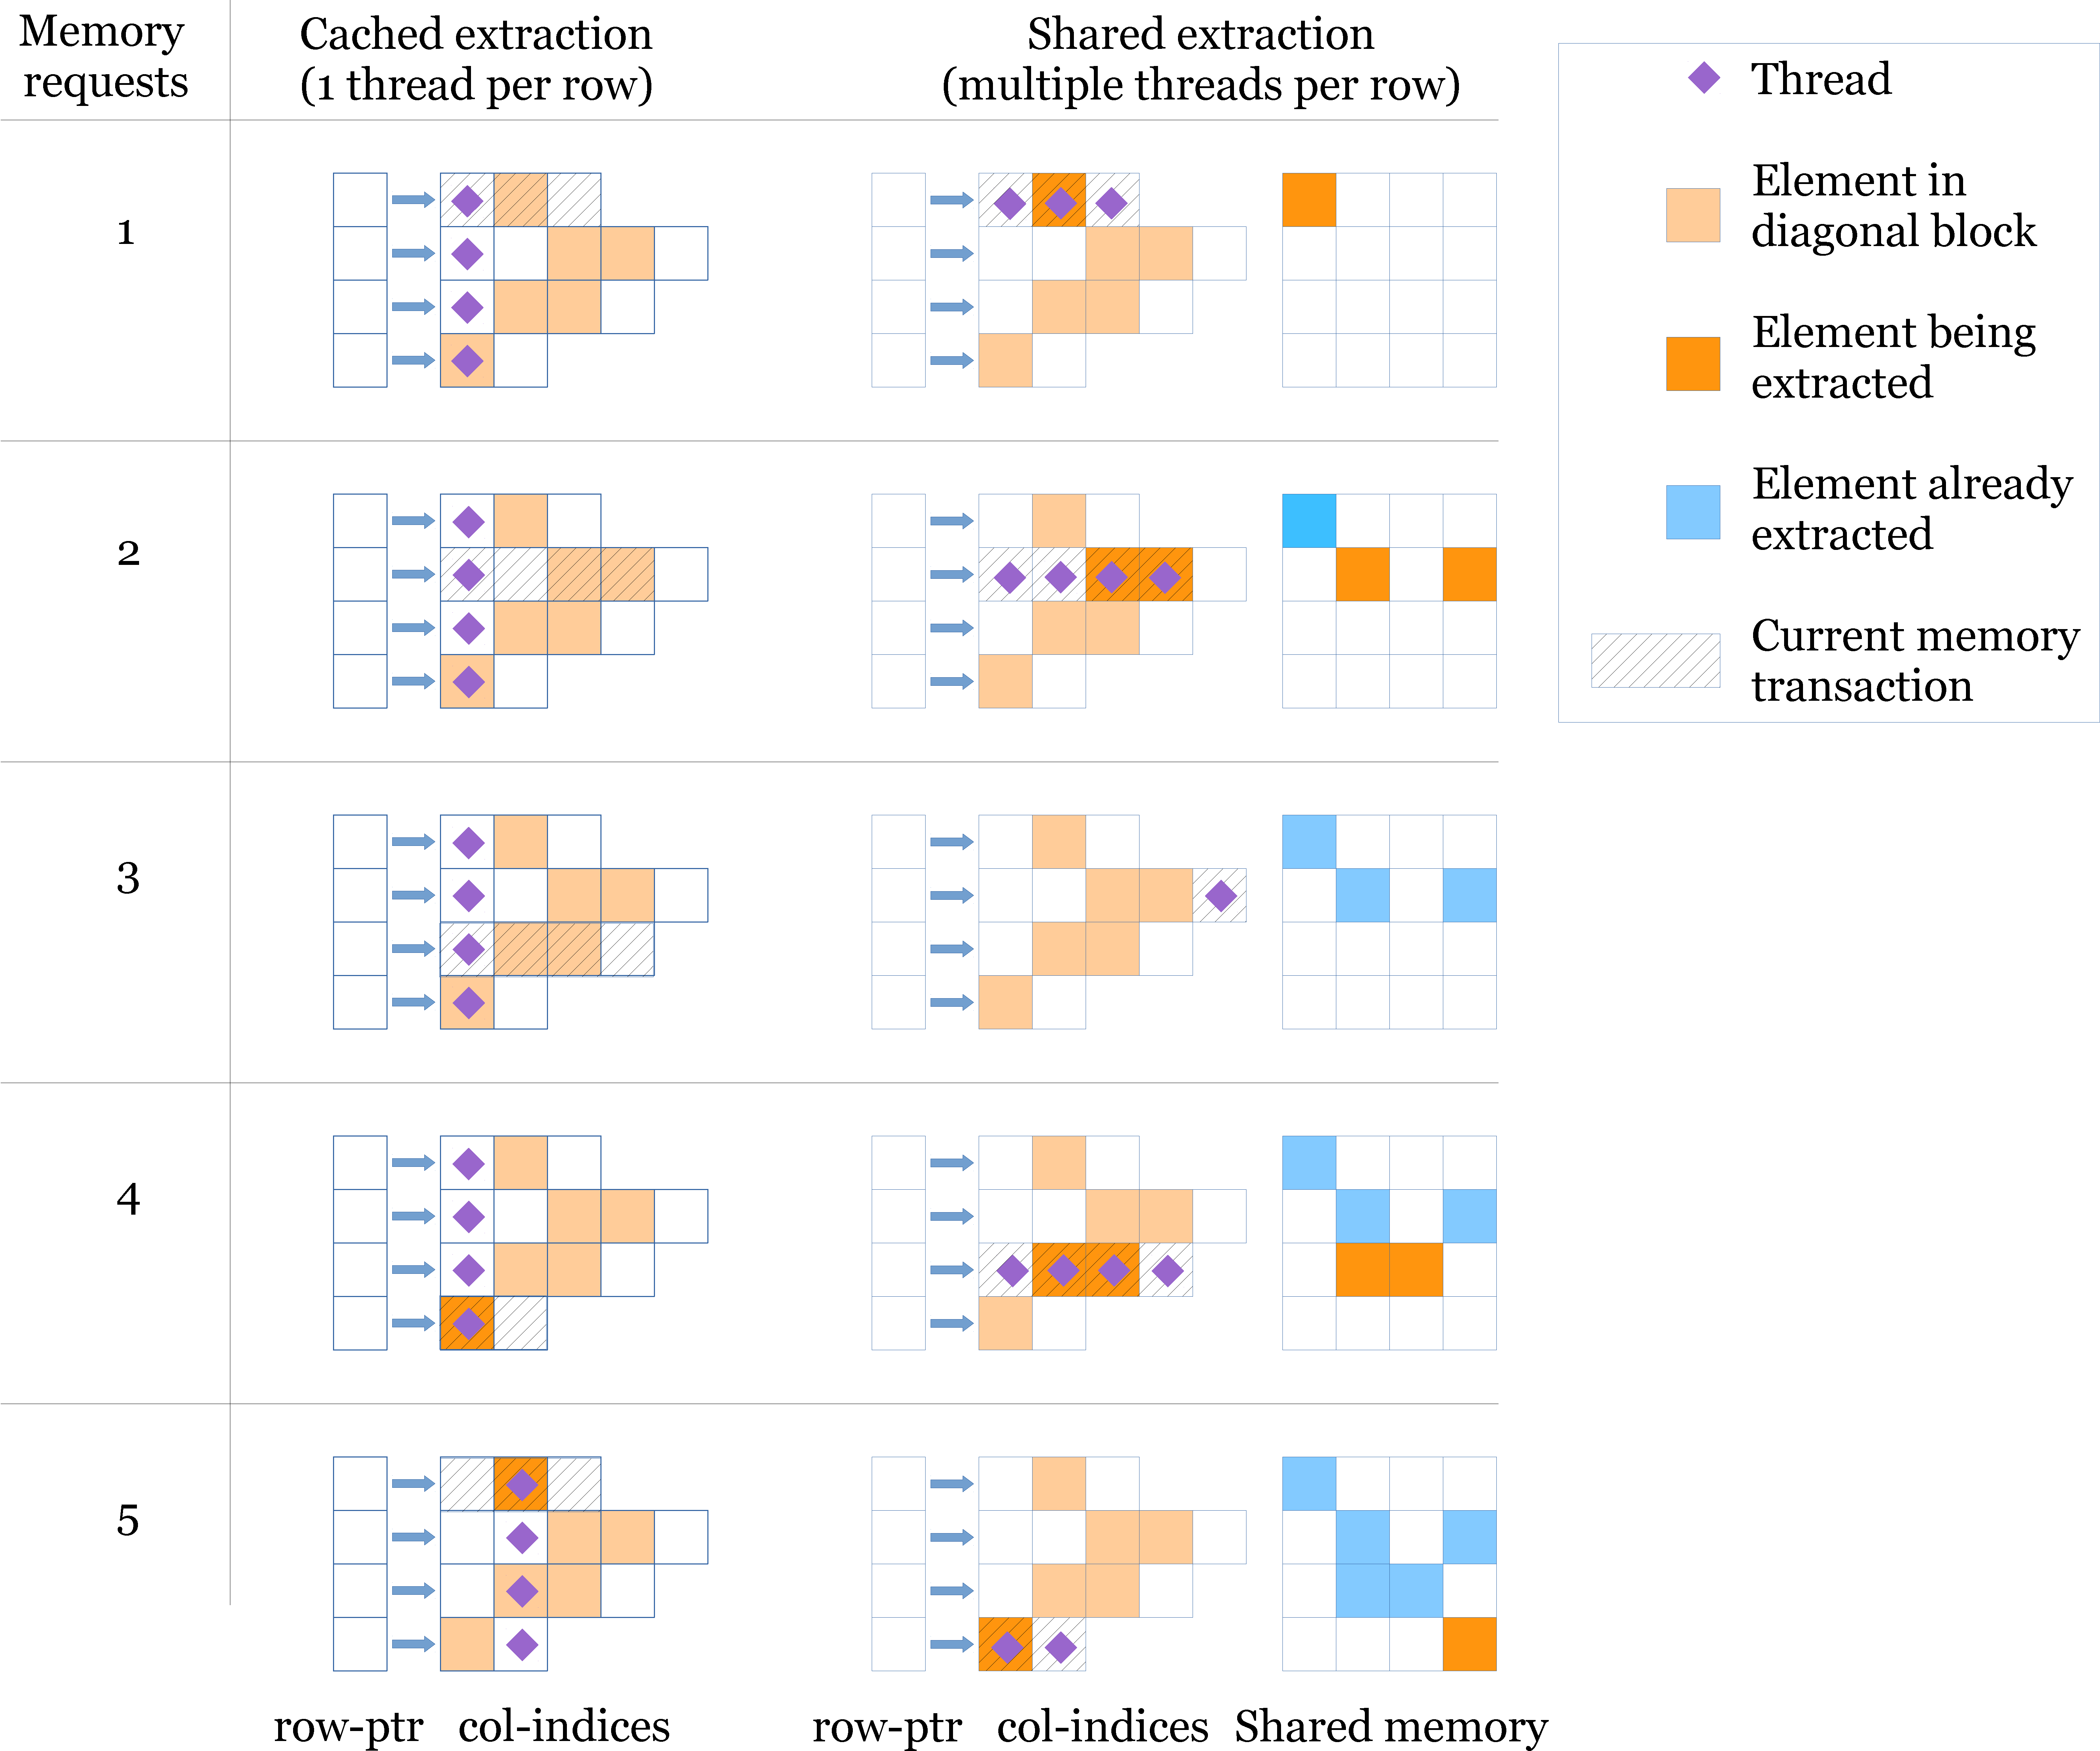
\includegraphics[width=.85\columnwidth]{plots/shared_extraction_legend}
\end{tabular}
\end{center}
\caption
[Illustration of the memory requests for the cached extraction and shared
extraction]
{Illustration of the memory requests for the cached extraction and shared extraction (left and right, respectively).
We assume warps of 4 threads and memory transactions of 4 values.
We only show the accesses to the vector storing the {\sf col-indices} of the CSR matrix structure; 
the access to the actual values induces far less overhead,
as these memory locations are accessed only if a location belonging to a diagonal block is found.
In that case, the access pattern is equivalent to the one used for {\sf col-indices}.
}
\label{2017-gje-block-jacobi:fig:memtransact}
\end{figure}

\subsection{Preconditioner application}
\label{2017-gje-block-jacobi:sec:precapply}
Once the block-inverse is generated,
the block-Jacobi preconditioner can be applied in terms 
of a sparse matrix-vector product
({\sc spmv}).

\vspace*{1ex}
\noindent
\textbf{Structure-aware  {\sc spmv}.}
We improve the performance of the block-Jacobi preconditioner by 
replacing the generic sparse matrix-vector product with a specialized kernel
that exploits the block structure of the preconditioner matrix.
In detail, we use a variable-size batched dense matrix-vector multiplication
({\sc gemv}) to multiply the distinct block inverses $D_i^{-1}$  
with the appropriate vector segments.
{As} in the preconditioner generation,
the blocks are distributed among the (sub-)warps,
with each (sub-)warp handling the multiplication for one vector segment.
In contrast to the elements of the matrix, which are all 
used for only a single multiplication,
the elements in the vector segment 
are reused in the multiplication with the distinct rows of the block.
Hence, it is beneficial to read the elements of the vector segment 
into the registers of the distinct threads of the (sub-)warp (one element per thread) 
at the beginning of the routine.
The performance of {{\sc gemv} is constrained} by the memory bandwidth.
It is therefore essential to ensure coalesced memory accesses
by forcing each (sub-)warp to read the diagonal blocks row-wise 
(the block-diagonal matrix is stored
in the row-major based CSR matrix format).
For each row of the block, the threads of the (sub-)warp then use
warp shuffles to compute the dot product of the matrix row and the 
vector entries they keep in registers.
Finally, the result is written to the appropriate position in the output vector.
